

\section{Cross Section Recommendations}\label{sec:recs}

The previous sections summarize the perturbative ingredients entering the current state-of-the-art prediction for Higgs boson pair production via gluon fusion. In this section we combine these results into the recommended reference cross sections, uncertainties, and invariant-mass distribution. Unless a dedicated alternative setup is required, the numbers reported here should be used for phenomenological studies and experimental interpretations.

\subsection[\texorpdfstring{NNLO$_{\textup{FTapprox}}$}{NNLO FTapprox}]{\texorpdfstring{\boldmath$\textup{NNLO}_{\textup{FTapprox}}$}{NNLO FTapprox}}

\begin{table}[htbp]
\begin{center}
\begin{tabular}{lccc}
\toprule
$\sqrt{s}$ [TeV] & \textbf{13} & \textbf{13.6} & \textbf{14} \\
\midrule
$\sigma$ [fb] & 30.75 & 34.01 & 36.27 \\\hline
$\pm$ PDF unc. [\%] & 1.96 & 1.92 & 1.89 \\
$\pm \alpha_s$ unc. [\%] & 1.51 & 1.49 & 1.47 \\
{\bfseries\boldmath $\pm$ PDF $+$ $\alpha_s$ unc. [\%]} & \textbf{2.47} & \textbf{2.43} & \textbf{2.39} \\\hline
QCD scale unc. [\%] & $^{+2.11}_{-4.98}$ & $^{+2.07}_{-4.85}$ & $^{+2.01}_{-4.78}$ \\
$\pm$ THU [\%] & 0.14 & 0.19 & 0.21 \\
\bottomrule
\end{tabular}
\caption{Total cross sections in $\textup{NNLO}_{\textup{FTapprox}}$~\cite{Grazzini:2018bsd}, at $13$, $13.6$ and $14\,\textup{TeV}$ proton centre-of-mass energies, with the Higgs boson mass set to $m_h = 125\,\textup{GeV}$. The central renormalization and factorization scale is taken to be $\mu_0  = m_{hh}/2$, and the scale uncertainties were obtained through a 7-point variation around $\mu_0$. The top quark mass was set to $m_t=173.0$~GeV and the bottom quark mass was set to zero, employing a 5-flavour scheme. The ``theory uncertainty'' (THU) only contains integration errors combined with $r_\mathrm{cut}\rightarrow 0$ extrapolation uncertainties. The PDF set \texttt{PDF4LHC21\ttus 40} was used. The PDF $+$ $\alpha_s$ uncertainty is obtained by adding the two contributions in quadrature.}
\label{tab:nnlo_ftapprox_xs_125}
\end{center}
\end{table}

The total cross sections in the $\textup{NNLO}_{\textup{FTapprox}}$ approximation~\cite{Grazzini:2018bsd} are shown in Table~\ref{tab:nnlo_ftapprox_xs_125} for proton centre-of-mass energies of 13, 13.6 and 14~TeV, with the Higgs boson mass set to $m_h = 125$~GeV. The central renormalization and factorization scale is taken to be $\mu_0  = m_{hh}/2$, and the scale uncertainties were obtained through a 7-point variation around $\mu_0$.
%The top mass was set to $m_t=173.0$~GeV. 
The top quark mass was set to $m_t=173.0$~GeV and the bottom quark mass was set to zero, employing a five-flavour scheme (5FS). The ``theory uncertainty'' (THU) contains integration errors combined with $r_\mathrm{cut}\rightarrow 0$ extrapolation uncertainties. The \texttt{PDF4LHC21\ttus 40} PDF set was used.

\subsection[\texorpdfstring{$\textup{N}^3\textup{LO}+\textup{N}^3\textup{LL}$ $K$-factors}{N3LO+N3LL K-factors}]{\texorpdfstring{\boldmath$\textup{N}^3\textup{LO}+\textup{N}^3\textup{LL}$ $K$-factors}{N3LO+N3LL K-factors}}

The N$^3$LO+N$^3$LL QCD $K$-factor~\cite{Chen:2019lzz,Ajjath:2022kpv} is defined as
\begin{equation}\label{eq:n3lokfac}
K_3 = \left(\frac{\mathrm{N^3LO+N^3LL~HTL} }{\mathrm{NNLO~HTL}}\right)\;.
\end{equation}

\begin{sloppypar}
The vacuum expectation value was set to $v=246.2197$~GeV. The corresponding Fermi constant was $G_F = 1.166378 \times 10^{-5}$~GeV$^{-2}$. The top quark mass was set to $m_t=173.0$~GeV. The central renormalization and factorization scale was taken to be $\mu_0  = m_{hh}/2$.
\end{sloppypar}

The uncertainty due to the use of an NNLO PDF instead of an N$^3$LO PDF is estimated via: 
\begin{equation}
 \Delta ^{\mathrm{MHOU}}_\mathrm{NNLO} =  \left| \frac { \sigma^{\mathrm{N}^3\mathrm{LO}}_{\mathrm{N}^3\mathrm{LO-PDF}} - \sigma^{\mathrm{N}^3\mathrm{LO}}_{\mathrm{NNLO-PDF}} } { \sigma^{\mathrm{N}^3\mathrm{LO}}_{\mathrm{N}^3\mathrm{LO-PDF}}  }  \right|\;,
 \label{eq:deltan3lopdf}
\end{equation}
where the N$^3$LO and NNLO PDFs used were the (approximate) \texttt{MSHT20xNNPDF40\ttus aN3LO\ttus qed} and \texttt{MSHT20xNNPDF40\ttus NNLO\ttus qed}, respectively.

\begin{table}[htbp]
\begin{center}
\begin{tabular}{lccc}
\toprule
$\sqrt{s}$ [TeV] & \textbf{13} & \textbf{13.6} & \textbf{14} \\
\midrule
$K_3$ & 1.030913 & 1.030812 & 1.030736 \\
$\Delta K_{3\rm down}/K_3$ [\%] & 9.3460 & 9.2396 & 9.1721 \\
$\Delta K_{3\rm up}/K_3$ [\%] & 4.9088 & 4.8756 & 4.8537 \\
$\Delta^{\mathrm{MHOU}}_{\mathrm{NNLO}}$ [\%] & 2.1207 & 2.1700 & 2.1799 \\
\bottomrule
\end{tabular}
\caption{$K$-factors $\mathrm{N^3LO{+}N^3LL}/\mathrm{NNLO}$ for the total cross section (relative uncertainties).}
\label{tab:kfactor_n3lo_n3ll_over_nnlo}
\end{center}
\end{table}

The total cross section results are shown in Table~\ref{tab:kfactor_n3lo_n3ll_over_nnlo}, including the upper and lower variations. The last row estimates the effect of missing higher-order corrections associated with using NNLO PDFs in the N$^3$LO calculation. This uncertainty is quoted for completeness, but is not combined in the final recommendation; the corresponding final uncertainty is inherited from the $\textup{NNLO}_{\textup{FTapprox}}$ calculation.


\subsection[\texorpdfstring{NLO Electroweak $K$-factors}{NLO Electroweak K-factors}]{\texorpdfstring{NLO Electroweak \boldmath$K$-factors}{NLO Electroweak K-factors}}

The $K$-factor due to NLO electroweak corrections is defined as
\begin{equation}\label{eq:NLOEWkfac}
K_\mathrm{EW} = \frac{\sigma_\mathrm{NLO~EW}}{\sigma_\mathrm{LO}} \;. 
\end{equation}

The input parameters were taken to be as in Ref.~\cite{Bi:2023bnq}:
\begin{itemize}
\item $m_t = 172.69$ GeV,
\item $m_h^2 / m_t^2 = 12 / 23 \Rightarrow m_h = 124.74$~GeV,
\item $m_Z^2 / m_t^2 = 23 / 83 \Rightarrow m_Z = 90.91$~GeV,
\item $m_W^2 / m_t^2 = 14 / 65 \Rightarrow m_W = 80.14$~GeV,
\item $G_F = 1.166378 \times 10^{-5}$~GeV$^{-2}$.
\end{itemize}
We note that the top and Higgs boson masses differ from those used in the $\textup{NNLO}_{\textup{FTapprox}}$ and N$^3$LO calculations. However, the $K$-factors are not particularly sensitive to these.

\begin{table}[htbp]
\begin{center}
\begin{tabular}{lccc}
\toprule
$\sqrt{s}$ [TeV] & \textbf{13} & \textbf{13.6} & \textbf{14} \\
\midrule
$K_\mathrm{EW}$ & 0.959 & 0.959 & 0.958 \\
\bottomrule
\end{tabular}
\caption{NLO electroweak $K$-factors for the total cross section, defined in Eq.~\eqref{eq:NLOEWkfac}, at $13$, $13.6$ and $14\,\textup{TeV}$.}
\label{tab:nlo_ew_kfac}
\end{center}
\end{table}

The NLO electroweak $K$-factors for the total cross section at 13, 13.6 and 14~TeV are shown in Table~\ref{tab:nlo_ew_kfac}. The scale variation uncertainties on these values are at the per-mille level or better, and therefore we do not include them here. We also note that at present, no electroweak effects are included in the PDF sets employed. 

\subsection{Combination}\label{subsec:combination}

The final recommended cross section is obtained by multiplying the $\textup{NNLO}_{\textup{FTapprox}}$ prediction by the N$^3$LO+N$^3$LL QCD $K$-factor and the NLO electroweak $K$-factor,
\begin{equation}\label{eq:xs_reco}
\sigma_\mathrm{rec.}(\sqrt{s}) \;=\; \sigma_{\textup{NNLO}_{\textup{FTapprox}}}(\sqrt{s}) \times K_3(\sqrt{s}) \times K_\mathrm{EW}(\sqrt{s}) \;,
\end{equation}
where $K_3$ and $K_\mathrm{EW}$ are given in Eqs.~\eqref{eq:n3lokfac} and~\eqref{eq:NLOEWkfac}, respectively. The central values are computed using the
central entries of Tables~\ref{tab:nnlo_ftapprox_xs_125},~\ref{tab:kfactor_n3lo_n3ll_over_nnlo} and~\ref{tab:nlo_ew_kfac}.

\paragraph{Scale and THU uncertainties.}
The final prediction combines information from the $\textup{NNLO}_{\textup{FTapprox}}$ calculation and from the N$^3$LO+N$^3$LL QCD $K$-factor. The scale variations of these two ingredients should therefore not be interpreted as independent uncertainties and combined again. For the final recommendation, we take the QCD scale uncertainty directly from the $\textup{NNLO}_{\textup{FTapprox}}$ prediction,
\begin{equation}
\delta_\mathrm{scale}^\mathrm{final}(\sqrt{s}) \;=\; \delta_{\mathrm{scale},\,\textup{NNLO}_{\textup{FTapprox}}}(\sqrt{s}) \;,
\end{equation}
as quoted in Table~\ref{tab:nnlo_ftapprox_xs_125}. The scale variation of the N$^3$LO+N$^3$LL $K$-factor is shown separately in Table~\ref{tab:kfactor_n3lo_n3ll_over_nnlo} and is not combined with the scale uncertainty of the final recommendation. No additional scale uncertainty is assigned to $K_\mathrm{EW}$ in this prescription. The THU assigned to the final recommendation, which accounts for the integration errors and $r_\mathrm{cut}\to0$ extrapolation uncertainties in the $\textup{NNLO}_{\textup{FTapprox}}$ calculation, is likewise taken from Table~\ref{tab:nnlo_ftapprox_xs_125}.

\paragraph{PDF and $\alpha_s$ uncertainties.}
The quantity $\Delta^{\mathrm{MHOU}}_\mathrm{NNLO}$ in Eq.~\eqref{eq:deltan3lopdf} estimates the possible effect of using NNLO PDFs in the N$^3$LO component, rather than a fully consistent N$^3$LO PDF set. We use this comparison only to assess the possible size of the PDF-order effect and do not add it to the final uncertainty budget. The quoted PDF and $\alpha_s$ uncertainties of the final recommendation are therefore inherited from the $\textup{NNLO}_{\textup{FTapprox}}$ calculation, as given in Table~\ref{tab:nnlo_ftapprox_xs_125}. Their combined contribution is obtained by adding the PDF and $\alpha_s$ uncertainties in quadrature.

\paragraph{Top quark mass scheme uncertainty.}
An additional uncertainty is assigned to the definition of the virtual top quark mass entering the top Yukawa coupling and the propagators, following the prescription of Ref.~\cite{Baglio:2020wgt} and the discussion in Section~\ref{sec:scheme-scale-uncertainties}. In this approach the NLO prediction obtained with the top quark pole mass is compared with predictions in the $\overline{\mathrm{MS}}$ scheme.
%, using the N$^3$LO relation between the pole and $\overline{\mathrm{MS}}$ masses and N$^3$LL evolution of $\overline{m}_t(\mu_t)$.

We obtain the corresponding NLO predictions with \texttt{ggxy}~\cite{Davies:2025qjr}, which provides the required total cross sections and differential distributions for the different top quark mass schemes. Specifically, we consider four predictions: with the top quark pole mass $m_t$, and with $\overline{\mathrm{MS}}$ mass $\overline{m}_t(\mu_t)$ with $\mu_t = \overline{m}_t$, $\mu_t = m_{hh}$, and $\mu_t = m_{hh}/4$ (i.e.~the latter two being a factor of two around the central renormalization and factorization scale $\mu_R=\mu_F=m_{hh}/2$). In \texttt{ggxy} we run at the highest available order, i.e.~at five-loop for the strong coupling $\alpha_s$ and the $\overline{\mathrm{MS}}$ mass, and four-loop for the conversion between the pole mass and the $\overline{\mathrm{MS}}$ mass. We then construct, in the $m_{hh}$ distribution, the bin-by-bin maximum and minimum across the four top quark mass schemes; the corresponding inclusive uncertainty is obtained by integrating the bin-wise extrema. We investigated several methods for the numerical integration: similarly to~Ref.~\cite{Baglio:2020ini}, with piecewise integration (Boole's rule~\cite{boole1880,Abramowitz1964} for $m_{hh} < 300$ GeV and the trapezoidal method for $m_{hh}>300$ GeV), as well as the trapezoidal method with finer bins and a continuous fit. The final uncertainties change by about 1\% depending on the method and binning used.

% The scale $\mu_t$ associated with the running mass is treated as an additional unphysical scale: in addition to the fixed choice $\mu_t=m_t$, it is varied in the range $m_{hh}/4 \leq \mu_t \leq m_{hh}$, i.e.\ by a factor of two around the central renormalization and factorization scale $\mu_R=\mu_F=m_{hh}/2$.

% For differential predictions the envelope is constructed bin by bin in $m_{hh}$, taking in each bin the maximum and minimum of the pole-mass and $\overline{\mathrm{MS}}$ predictions over the allowed $\mu_t$ choices; the corresponding inclusive variation is then obtained by integrating the bin-wise extrema. Since this uncertainty was found in Ref.~\cite{Baglio:2020wgt} to be approximately independent of the usual $\mu_R,\mu_F$ scale variation, we include it separately in the final uncertainty table.

\paragraph{Final recommendations.}
The resulting central values and uncertainties are summarized in Table~\ref{tab:final_xs_reco_125} for $\sqrt{s}=13, 13.6, 14$~TeV, including the top quark mass scheme uncertainty and its linear combination with the scale and THU uncertainties. For the additional choices of the Higgs boson mass shown in Table~\ref{tab:final_xs_reco_125_mh}, we use \texttt{ggxy}~\cite{Davies:2025qjr} to compute the NLO cross section at the target value of $m_h$ and at $m_h=125$~GeV with the same setup. We then form the ratio $\sigma_{\mathrm{NLO}}(m_h)/\sigma_{\mathrm{NLO}}(125~\mathrm{GeV})$ at each centre-of-mass energy and multiply the corresponding $m_h=125$~GeV final recommendation by this factor.

\begin{table}[htbp]
\begin{center}
\begin{tabular}{lccc}
\toprule
$\sqrt{s}$ [TeV] & \textbf{13} & \textbf{13.6} & \textbf{14} \\
\midrule
$\sigma_\mathrm{rec.}$ [fb] & 30.40 & 33.62 & 35.81 \\\hline
$\pm$ PDF unc. [\%] & 1.96 & 1.92 & 1.89 \\
$\pm \alpha_s$ unc. [\%] & 1.51 & 1.49 & 1.47 \\
{\bfseries\boldmath $\pm$ PDF $+$ $\alpha_s$ unc. [\%]} & \textbf{2.47} & \textbf{2.43} & \textbf{2.39} \\\hline
QCD scale unc. [\%] & $^{+2.11}_{-4.98}$ & $^{+2.07}_{-4.85}$ & $^{+2.01}_{-4.78}$ \\
$m_t$ scheme unc. [\%] & $^{+5}_{-16}$ & $^{+5}_{-16}$ & $^{+5}_{-16}$ \\
$\pm$ THU [\%] & 0.14 & 0.19 & 0.21 \\
{\bfseries\boldmath Scale $+$ THU $+$ $m_t$ scheme unc. [\%]} & {\bfseries\boldmath $^{+7.25}_{-21.12}$} & {\bfseries\boldmath $^{+7.26}_{-21.04}$} & {\bfseries\boldmath $^{+7.22}_{-20.99}$} \\
\bottomrule
\end{tabular}
\caption{Final recommended inclusive total cross sections for Higgs boson pair production via gluon fusion obtained using Eq.~\eqref{eq:xs_reco}.
The QCD scale and THU uncertainties, as well as the $\alpha_s$ and PDF uncertainties, are taken directly from the $\textup{NNLO}_{\textup{FTapprox}}$ prediction (Table~\ref{tab:nnlo_ftapprox_xs_125}). The PDF $+$ $\alpha_s$ uncertainty is obtained by adding the two contributions \textit{in quadrature}. The final combined scale, THU and $m_t$ scheme uncertainty is obtained by adding the corresponding components \textit{linearly}.}
\label{tab:final_xs_reco_125}
\end{center}
\end{table}

\begin{table}[htbp]
\centering
\begin{tabular}{@{}lccc@{}}
\toprule
& \multicolumn{3}{c}{$\sigma_{\mathrm{rec.}}$ [fb]} \\
\cmidrule(lr){2-4}
$m_h$ [GeV] & $\sqrt{s}=13$~TeV
& $\sqrt{s}=13.6$~TeV
& $\sqrt{s}=14$~TeV \\
\midrule
124.8 & 30.48 & 33.68 & 35.90 \\
125 & 30.40 & 33.62 & 35.81 \\
125.2 & 30.29 & 33.54 & 35.68 \\
\bottomrule
\end{tabular}
\caption{Inclusive cross sections for Higgs boson pair production via gluon fusion
at different values of $m_h$, obtained from those at $m_h = 125$~GeV after rescaling
with the ratio $\sigma_{\mathrm{NLO}}(m_h)/\sigma_{\mathrm{NLO}}(125~\mathrm{GeV})$
for centre-of-mass energies of 13, 13.6, and 14~TeV.}
\label{tab:final_xs_reco_125_mh}
\end{table}


\subsection{Higgs Boson Pair Invariant-Mass Distribution}\label{subsec:mhh_distribution}
The recommended differential distribution in the Higgs boson pair invariant mass, $m_{hh}$, is constructed bin by bin following the multiplicative prescription of Eq.~\eqref{eq:xs_reco}. The $\textup{NNLO}_{\textup{FTapprox}}$ spectrum is multiplied by the differential QCD factor $K_3$ and the electroweak factor $K_\mathrm{EW}$, while the uncertainty band is inherited from the $7$-point scale variation of the $\textup{NNLO}_{\textup{FTapprox}}$ calculation. The top quark mass scheme uncertainty quoted in Table~\ref{tab:final_xs_reco_125} is not included in this differential uncertainty band.

The ratio inset in Fig.~\ref{fig:xs_vs_mhh_combination_14} shows $K_3$, $K_\mathrm{EW}$ and their product, making explicit the bin-wise rescaling applied to the $\textup{NNLO}_{\textup{FTapprox}}$ spectrum.

The shape of the recommended spectrum and of the correction factors changes only mildly between the 13, 13.6 and 14~TeV centre-of-mass energies considered here. We therefore show the 14~TeV result as a representative case in Fig.~\ref{fig:xs_vs_mhh_combination_14}. The corresponding binned data files and the 13 and 13.6~TeV distributions are available from the LHC Higgs WG4 wiki~\cite{wg4wiki}.

%\begin{figure*}[htbp]
%\centering
%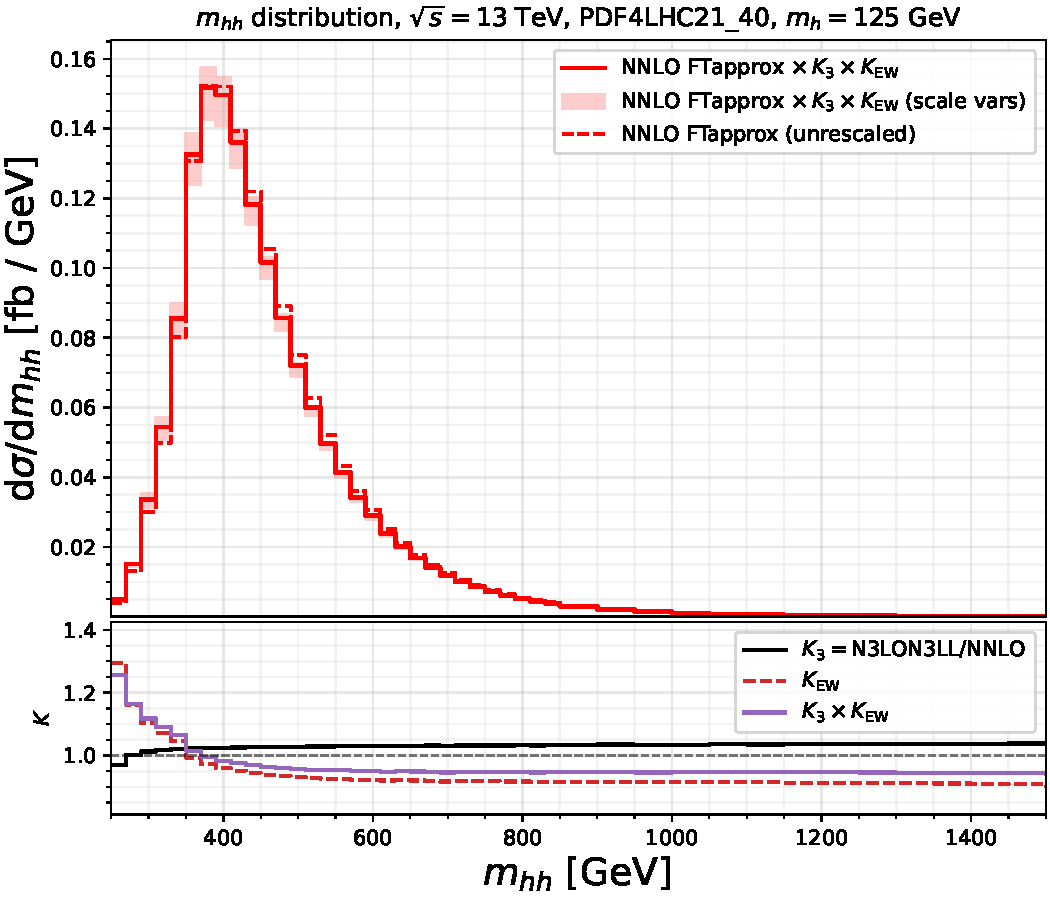
\includegraphics[width=0.8\textwidth]{Recommendations/COMBINATION_Mhh_13TeV_PDF4LHC21_40_mH125.pdf}
%\\
%\caption{Invariant-mass distributions for Higgs boson pair production at $\sqrt{s}=13$ TeV, including the N$^3$LO+NLL/NNLO and NLO EW $K$-factors (solid red). The unrescaled NNLO FTapprox is represented by the red-dashed line. The red error bands stem from $7$-point scale variations of the NNLO FTapprox calculation. The lower panel shows the $K$-factors N$^3$LO+NLL/NNLO and NLO EW $K$-factors, as well as their product.}
%\label{fig:xs_vs_mhh_combination_13}
%\end{figure*}

\begin{figure*}[htbp]
\centering
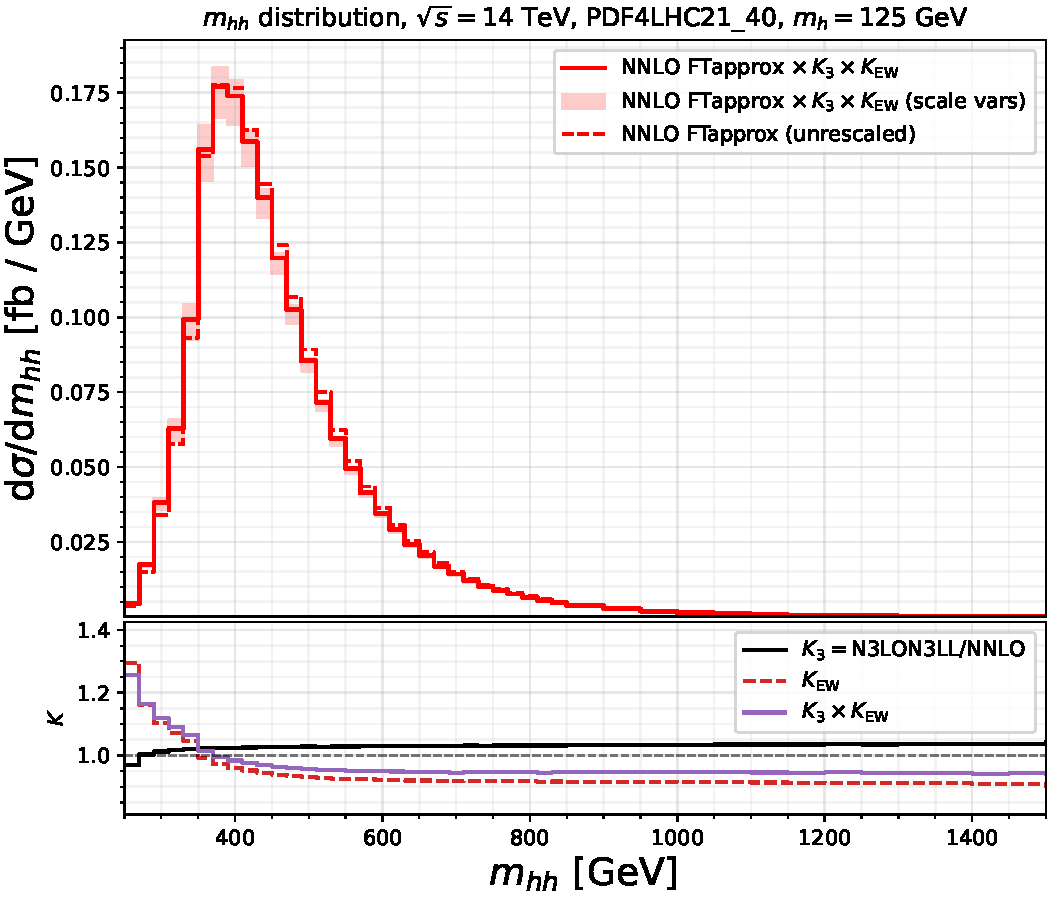
\includegraphics[width=0.9\textwidth]{Recommendations/COMBINATION_Mhh_14TeV_PDF4LHC21_40_mH125.pdf}
\\
\caption{Recommended Higgs boson pair invariant-mass distribution at $\sqrt{s}=14$~TeV. The solid red curve in the main panel is the final spectrum obtained by multiplying the $\textup{NNLO}_{\textup{FTapprox}}$ distribution by the differential N$^3$LO+N$^3$LL/NNLO QCD and NLO EW $K$-factors. The dashed red curve shows the unrescaled $\textup{NNLO}_{\textup{FTapprox}}$ input, and the red band gives the inherited $7$-point scale variation of the $\textup{NNLO}_{\textup{FTapprox}}$ calculation. The ratio inset shows the QCD factor $K_3=\textup{N}^3\textup{LO}+\textup{N}^3\textup{LL}/\textup{NNLO}$, the electroweak factor $K_\mathrm{EW}$, and their product.}
\label{fig:xs_vs_mhh_combination_14}
\end{figure*}

%\begin{figure*}[htbp]
%\centering
%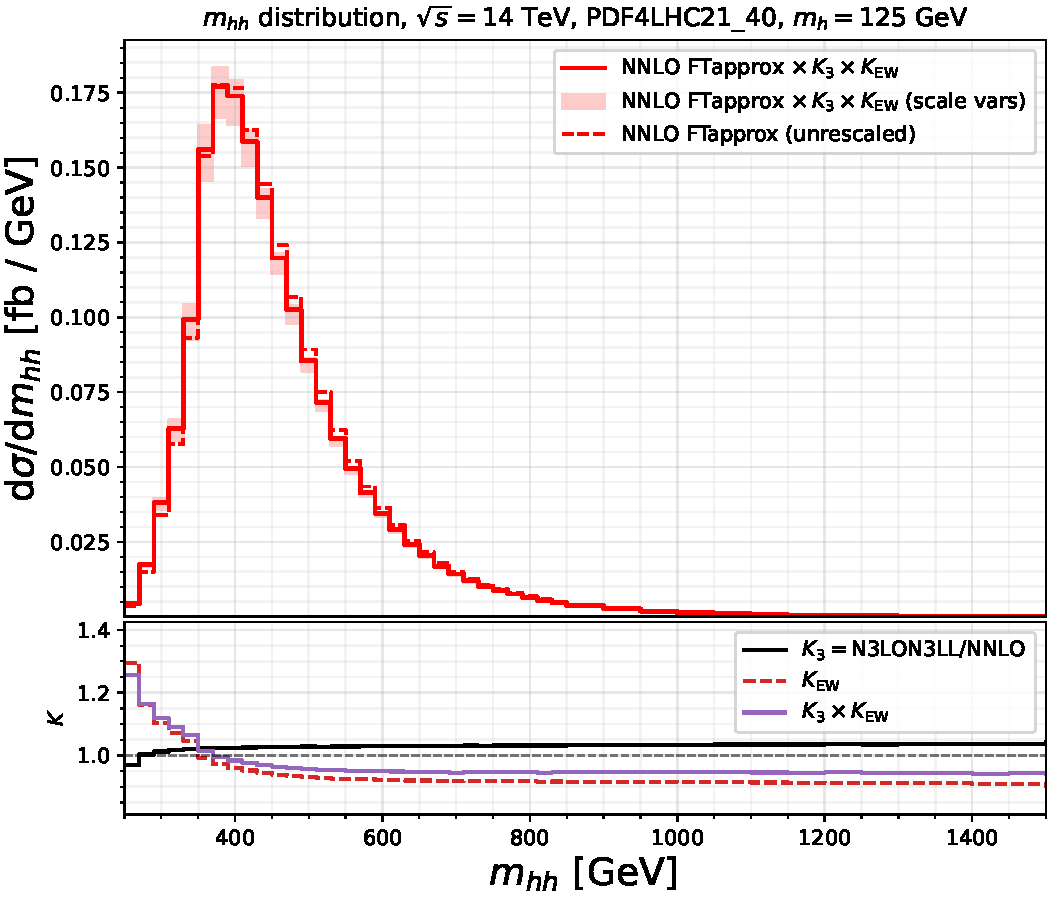
\includegraphics[width=0.8\textwidth]{Recommendations/COMBINATION_Mhh_14TeV_PDF4LHC21_40_mH125.pdf}
%\\
%\caption{Invariant-mass distributions for Higgs boson pair production at $\sqrt{s}=14$ TeV, including the N$^3$LO+NLL/NNLO and NLO EW $K$-factors (solid red). The unrescaled NNLO FTapprox is represented by the red-dashed line. The red error bands stem from $7$-point scale variations of the NNLO FTapprox calculation. The lower panel shows the $K$-factors N$^3$LO+NLL/NNLO and NLO EW $K$-factors, as well as their product.}
%\label{fig:xs_vs_mhh_combination_14}
%\end{figure*}
